\section{Grundlagen}
\label{sec:grundlagen}
In diesem Versuch werden verschiedene Schaltungen mit Hilfe des
Operationsverstärkers realisiert.
Zunächst wird auf die physikalischen Eigenschaften eingegangen,
woraufhin verschiedene Schaltungen skizziert und schließlich
realisiert werden.

\subsection{Eigenschaften des Operationsverstärkers}
\label{subsec:eigenschaften}
Die wichtigste elektrische Eigenschaft des Operationsverstärkers
ist die Proportionalität der Ausgangsspannung $U_\text{A}$ zur
Differenz der Eingangsspannungen $U_\text{p}$ und $U_\text{N}$:
\begin{equation}
\label{eq:proportionalität}
    U_\text{A} = V(U_\text{p} - U_\text{N})\,,
\end{equation}
wobei $V$ die Verstärkungsspannung bezeichnet.

Aus technischer Sicht entspricht der Operationsverstärker einem
gleichstromgekoppeltem Differenzverstärker. Er ist in Abbildung
\ref{fig:op} dargestellt.
\begin{figure}
    \centering
    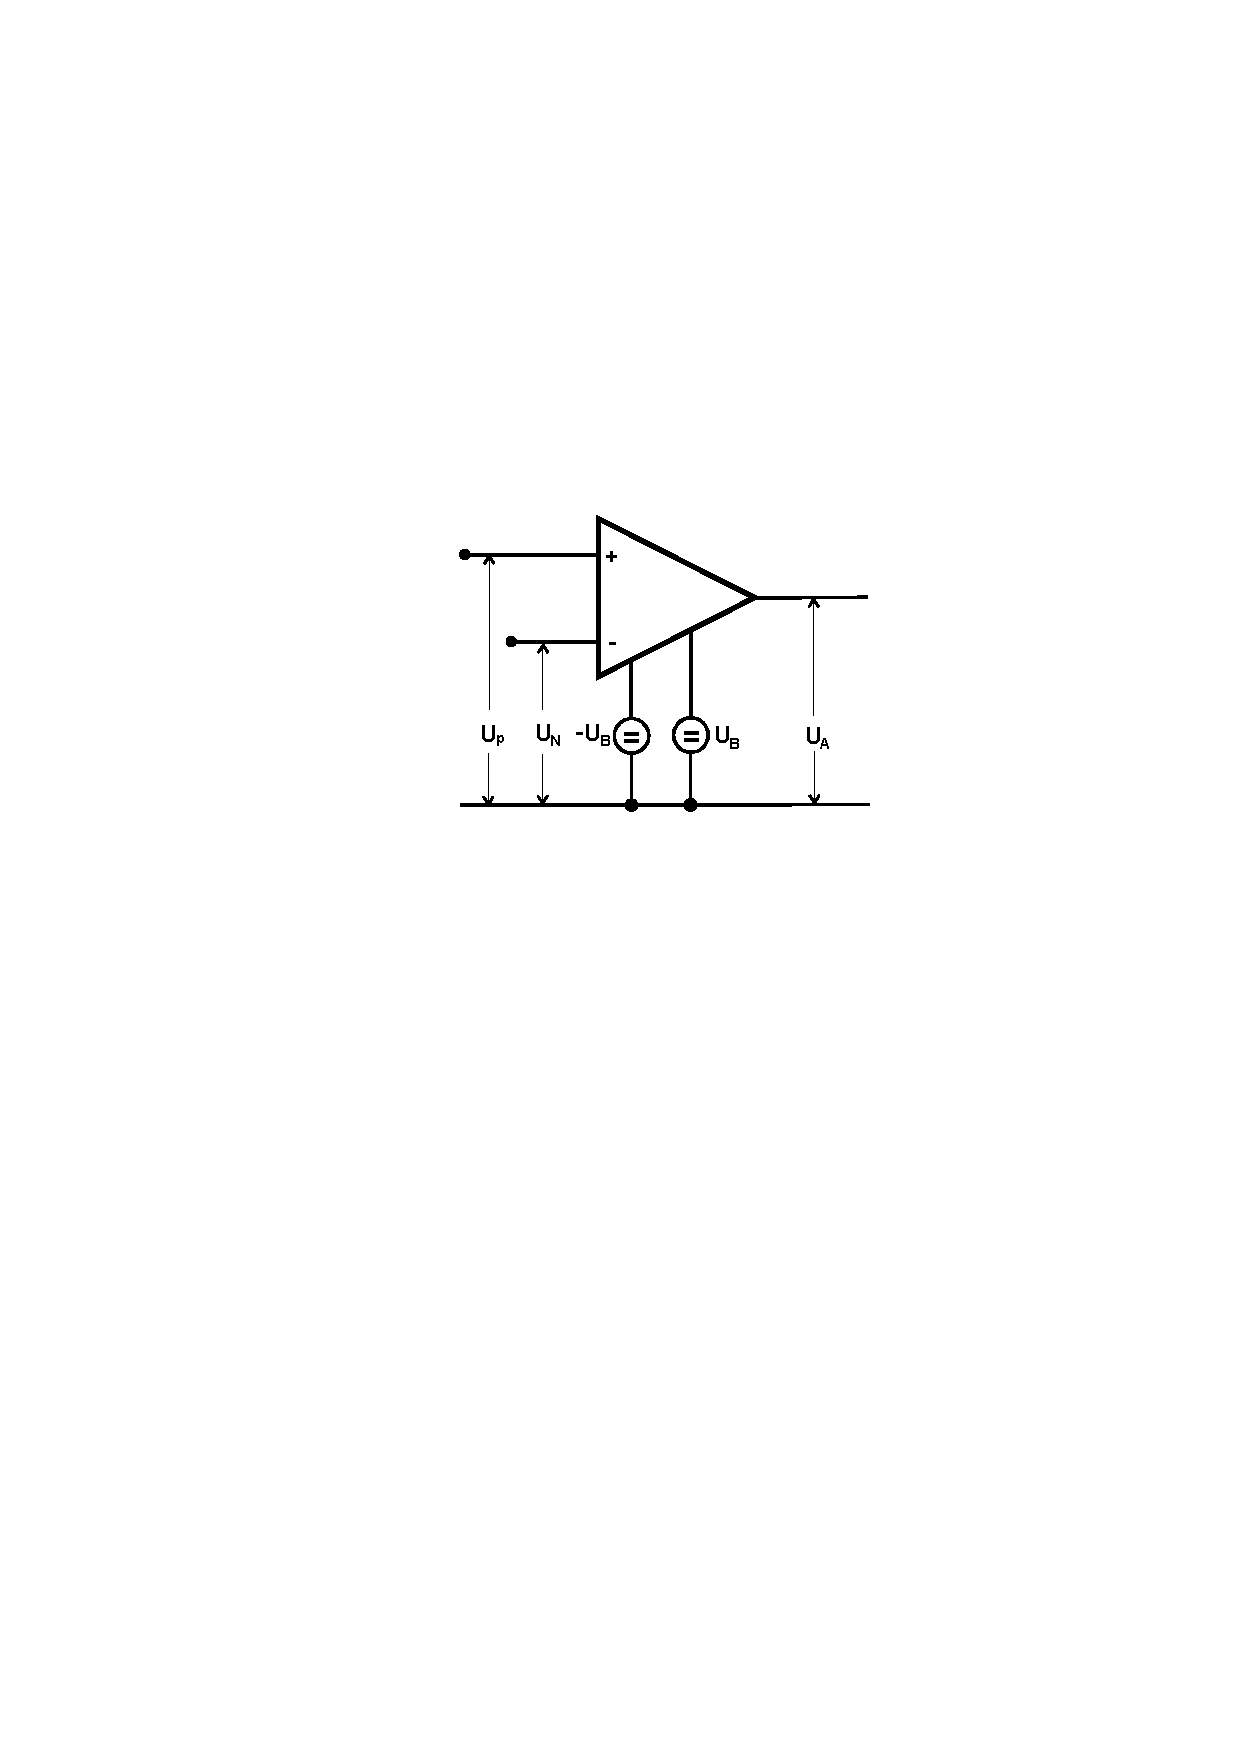
\includegraphics[width=0.7\linewidth]{img/op.pdf}
    \caption{
        Schaltbild eines Operationsverstärkers mit Ausgangsspannung
        $U_\text{A}$ und Eingangsspannungen $U_\text{p}$ und
        $U_\text{N}$ \cite{V51}.
    }
    \label{fig:op}
\end{figure}
